\documentclass[11pt,letterpaper]{article}
\usepackage[margin=1in]{geometry}
\usepackage{graphicx,booktabs,tabularx,siunitx,hyperref}
\hypersetup{hidelinks}
\setcounter{secnumdepth}{0}
\begin{document}
\subsubsection{Layer-specific stimuli and supported stepping in the bilateral W2L model}

\noindent\textbf{Methods.}
I evaluated the bilateral W2L controller with 108 graded neurons, 216 chemical connections, and 12 antagonist Hill-type muscle actuators. The controller included heel and toe contact channels, 12 homonymous type-II muscle-length channels for hip, knee, and ankle flexors and extensors bilaterally, and four retained phase-related type-II channels. Compiled neural and muscle calculations were coupled to MuJoCo with a \qty{0.2}{\milli\second} neural step and a \qty{2}{\milli\second} mechanical step. In suspended trials, I applied the same \qty{-10}{\nano\ampere}, \qty{100}{\milli\second} pulse separately to the left extensor RG, hip PF, and hip MN. Each response was compared with an unperturbed run of the same controller over a common interval (Figure~\ref{fig:w2l108_layer_stimuli}).

For ground tests, a passive sliding guide assembly permitted forward motion while limiting lateral displacement and rotation through physical contacts. I first selected a near-flat initial pose by inverse kinematics and then exchanged four mirrored PF-to-ankle-MN targets after checking the corresponding muscles' mechanical actions. These changes preceded fitting. A bounded Rustuna search varied a shared PF-to-MN recruitment factor and the bilateral toe-to-ankle-MN conductance. Accepted trials required repeated whole-foot clearance with unloading, opposite-foot support, alternating swing transitions, positive knee flexion, and maintained pelvis height. The objective combined measured assistance with impact-force and progression penalties.

\noindent\textbf{Results.}
The layered stimulus responses differed. The RG pulse produced a large local voltage excursion and changed subsequent PF, MN, and joint trajectories. The PF pulse changed downstream activity and joint motion while leaving the RG pattern comparatively close to baseline. The same MN pulse produced a smaller movement difference.

Correcting the initial pose increased qualified left/right swings from 3/1 to 7/8 and reduced mean net assistance from 89.25\% to 46.66\% of body weight (Table~\ref{tab:w2l108_ground_changes}). The ankle phase correction produced 9/8 qualified swings, 100\% alternating transitions, and 42.24\% assistance. All 24 bounded fitting trials met the acceptance criteria. The selected configuration retained 9/8 swings and 100\% alternation while reducing assistance to 39.24\%. Minimum knee flexion remained positive at \qty{2.50}{\degree} on the left and \qty{2.29}{\degree} on the right. Figure~\ref{fig:w2l108_ground} shows repeated unloading and clearance alongside joint motion and measured support.

\noindent\textbf{Discussion.}
These experiments separate initial-pose and muscle-action corrections from subsequent parameter fitting. The pose correction restored heel participation without increasing sensory gains, and the ankle correction aligned the shared PF drive with the muscles' verified actions. The remaining assistance and sharp contact-force peaks provide measurable targets for further training. The fitted objective measures support and mechanical loading; it does not estimate metabolic expenditure. Layer-specific stimuli provide a complementary test of how a controller's internal organization affects movement.

\begin{table}[htbp]
\centering
\caption{Changes in supported stepping after initial-pose correction, ankle phase correction, and bounded controller fitting. Swing counts and alternation are evaluated from 1 to 10 s; assistance is the mean net vertical support force over the full 10 s, normalized by model body weight.}
\label{tab:w2l108_ground_changes}
\small
\begin{tabularx}{\textwidth}{@{}Xrrr@{}}
\toprule
Condition & \shortstack{Swings\\L/R} & \shortstack{Alternation\\(\%)} & \shortstack{Assistance\\(\% BW)} \\
\midrule
Toe-down initial pose & 3/1 & 33.33 & 89.25 \\
Near-flat IK pose & 7/8 & 92.86 & 46.66 \\
IK + ankle phase correction & 9/8 & 100.00 & 42.24 \\
IK + phase correction + fitting & 9/8 & 100.00 & 39.24 \\
\bottomrule
\end{tabularx}
\end{table}

\begin{figure}[p]
\centering
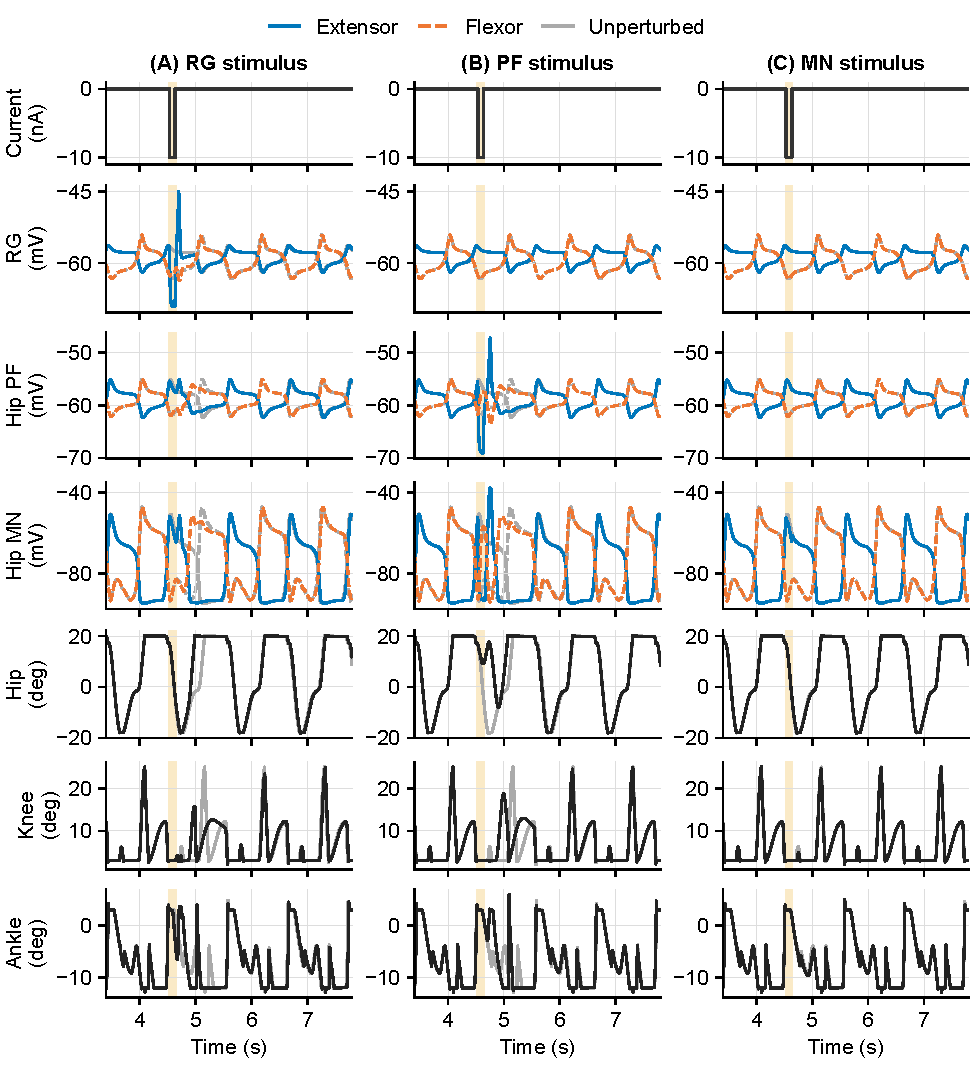
\includegraphics[width=\textwidth]{W2L108_left_RG_PF_MN_stimuli.pdf}
\caption[Layer-specific stimulation in the bilateral W2L controller]{Left-leg responses to separate extensor RG (A), hip PF (B), and hip MN (C) stimuli in the suspended W2L model. Each pulse is \qty{-10}{\nano\ampere} for \qty{100}{\milli\second}, beginning at \qty{4.534}{\second}; the top row shows the actual applied current, and shading marks its duration. Blue solid and orange dashed traces identify the named extensor and flexor neural pathways. Gray traces show the same neurons and joint angles without the test pulse; their solid and dashed neural traces retain the antagonist identities. Joint responses are black. The three columns use identical row scales and time limits. Neural voltages are recorded graded membrane potentials; joint angles retain the source anatomical convention, including positive knee flexion.}
\label{fig:w2l108_layer_stimuli}
\end{figure}

\begin{figure}[p]
\centering
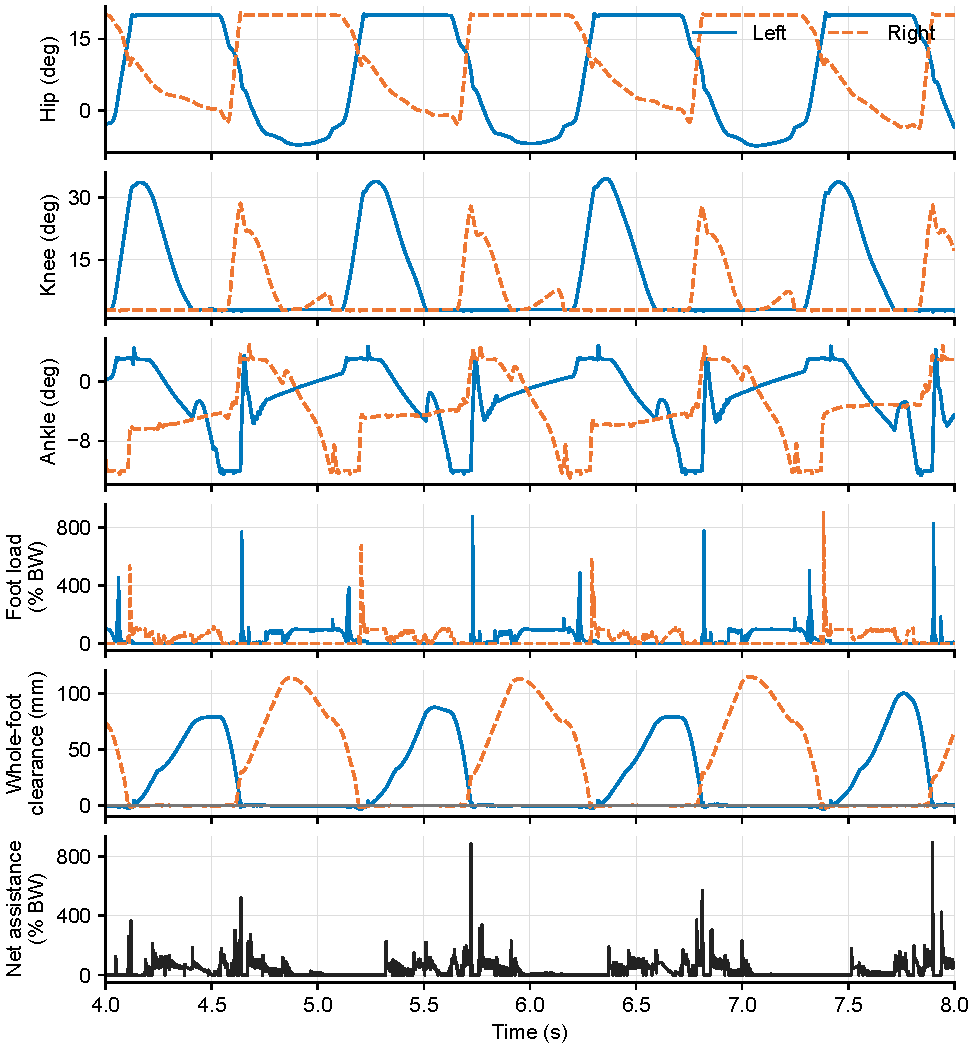
\includegraphics[width=\textwidth]{W2L108_tuned_ground_motion_load.pdf}
\caption[Supported stepping after W2L pose, phase, and gain corrections]{Joint motion, vertical foot load, minimum whole-foot clearance, and measured net vertical assistance in the fitted bilateral W2L configuration. Blue solid and orange dashed curves identify the left and right legs. The support apparatus consists of passive rails and a sliding guide with \qty{30}{\milli\meter} clearance. Assistance is the signed sum of measured rail, guide, and harness vertical reactions, divided by model body weight; the harness contribution is zero in this trial. The displayed interval retains the impact transients. Acceptance and assistance values in Table~\ref{tab:w2l108_ground_changes} are calculated over their stated scoring intervals rather than this plotted subset.}
\label{fig:w2l108_ground}
\end{figure}

\clearpage
\begin{figure}[p]
\centering
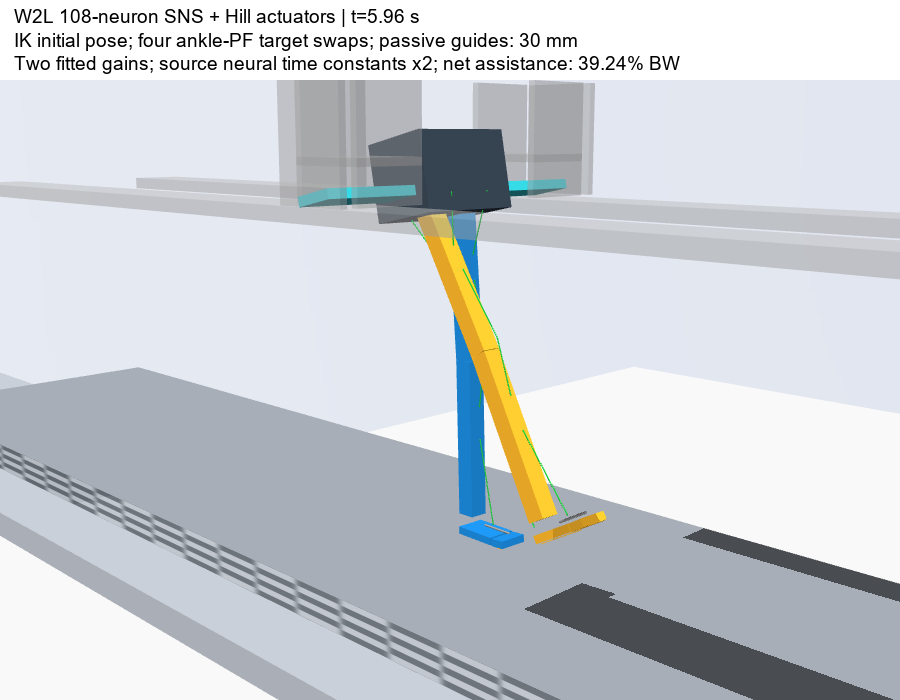
\includegraphics[width=\textwidth]{W2L108_tuned_ground_still.png}
\caption{The fitted W2L model during a recorded right-leg swing. The cyan root wings rest on passive support rails; transparent geometry shows the guide assembly. This frame is from the same fitted configuration as Figure~\ref{fig:w2l108_ground}.}
\end{figure}
\end{document}
